\documentclass{article}
\usepackage{graphicx}
\begin{document}
	\section*{Lsg Vorschlag LAÜ08 Maximmilian Maag}
	\subsection*{Aufgabe A}
	\subsection*{Aufgabe B}
	\subsection*{Aufgabe 1}
	\begin{tabular}{c|c|c}
		Matrix & Abbildung & Abbildungsgleichungen \\
		\hline
		M1&Spiegelung an der X-Achse& x' = x; y' = -y \\
		M2&Streckung um den Faktor 2& x' = 2x; y' = 2y \\
		M3&  & x' = -y; y' = x \\
		M4&& x' = 0; y' = - $\frac{1}{2}x$  + y \\
		M5&Projektion in die XY-Ebene& x' = 0; y' = y\\
		M6&Fix& x' = y; y' = x \\
		M7& Enthält Streckung und...  & x' = -3y; y' = 3x \\
		M8& Spiegelung an der X-Achse & x' = x; y' = -y; z' = z\\
		M9& Projektion in die XY-Ebene & x' = x; y' = y; z' = 0 \\
	\end{tabular}
	\subsection*{Aufgabe 2}
	Die Spalten der Matrix bilden die Bilder der Einheitsmatrix. Für die Matrix A ergeben sich daher folgende Abbildungen der Einheitsvektoren: \\
	\\
	$A = 
	\left(
	\begin{array}{ccc}
	-1&0& 0\\0 &1&0 \\ 0 & 0& 1
	\end{array}
	\right)$ \\
	$
	P'_{1} = 
	\left(\begin{array}{c}
	-1 \\0 \\0
	\end{array}\right)$ \\
	$
	P'_{2} = 
	\left(\begin{array}{c}
	0 \\ 1 \\ 0
	\end{array}\right)$ \\
	$
	P'_{3} = 
	\left(\begin{array}{c}
	0 \\ 0 \\ 1
	\end{array}\right)$ \\ \\
	Daraus Folgt $\vec{x}' = 
	\left(\begin{array}{c}
	-x\\y\\z
	\end{array}\right)$ \\
	Daraus lässt sich eine Spiegelung an der Y-Achse ableiten. \\
	Analog lässt sich aus der Matrix B folgender $\vec{x}'$ ablesen. \\ \\
	$\vec{x}' =  \left(\begin{array}{c}
	x \\ -y \\ z
	\end{array}\right)$ \\
	\\
	C = 
	$
	\left(
	\begin{array}{ccc}
	-1&0& 0\\0 &1&0 \\ 0 & 0& 1
	\end{array}
	\right)
	\cdot
	\left(
	\begin{array}{ccc}
	1&0& 0\\0 &-1&0 \\ 0 & 0& 1
	\end{array}
	\right)
	$ \\
	$
	C = 
	\left(
	\begin{array}{ccc}
	-1&0& 0\\0 &-1&0 \\ 0 & 0& 1
	\end{array}
	\right)
	$ \\ \\
	Aus C lässt sich eine Spiegelung entlang einer diagonalen Geraden durch den Ursprung ablesen.
	\subsection*{Aufgabe 3}
	
		det
	$\left(
	\begin{array}{cccc}
	1&2&3&4  \\ 2&0&2&0 \\ 4&7&1&1 \\  5&6&7&8
	\end{array}	
	\right)
	=
	-2 \cdot
	\left\|+
	\begin{array}{ccc}
	2&3&4 \\ 7&1&1 \\ 6&7&8
	\end{array}
	\right\|
	+ 0
	-2 \cdot
	\left\|
	\begin{array}{ccc}
	1&2&4 \\ 4&7&1 \\ 5&6&8
	\end{array}
	\right\|
	+ 0
	$ \\
	$-2 \cdot (16 + 18 + 196 -24 -14 -168) -2 \cdot (56+10+96-140-6-64)$ \\
	= 48
	\section*{Material}
	Hier finden sich Skizzen Tipps und Tricks. \\
	\section*{Material 1}
	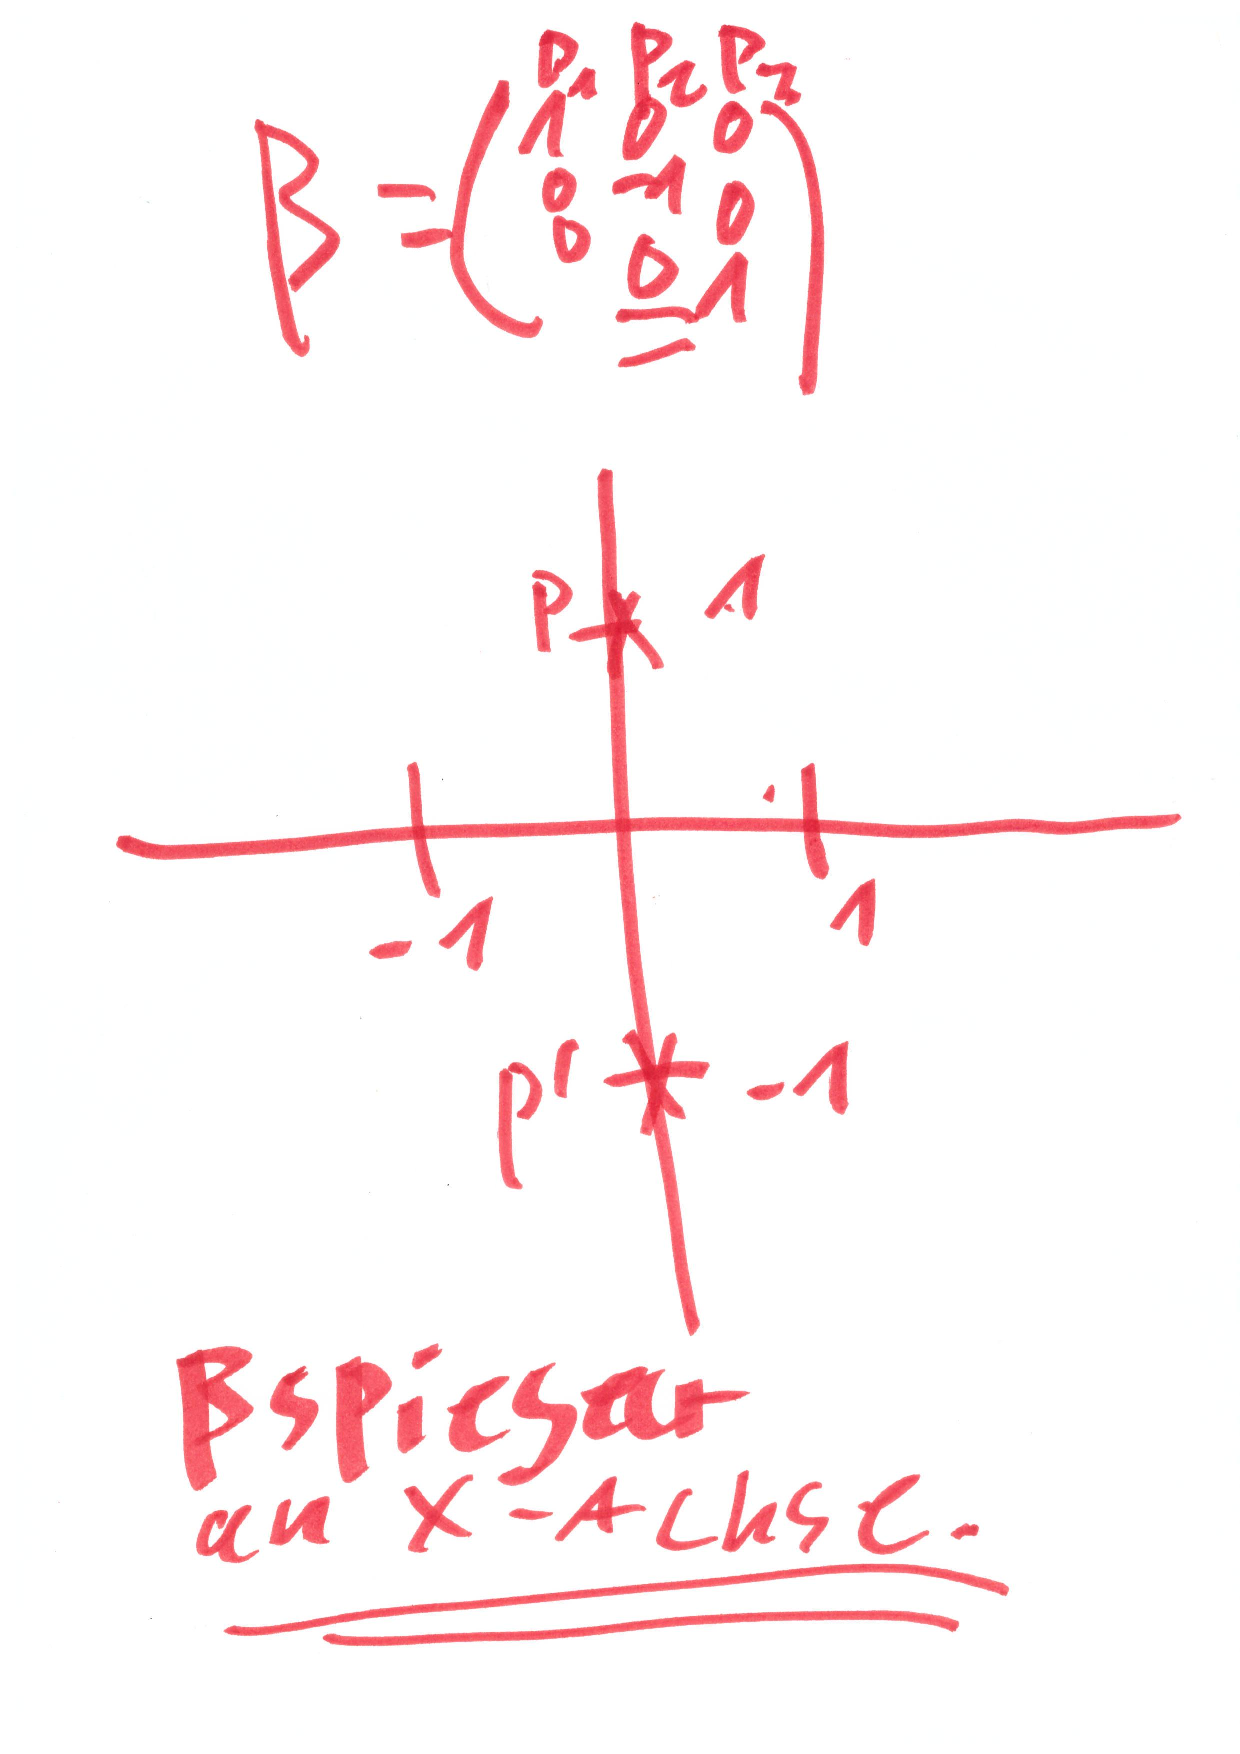
\includegraphics[width=\linewidth]{080201} \\
	Die Spalten der Matrix bilden die Bilder der Einheitsvektoren. Dieser Satz illustriert dargestellt zeigt eine Spiegelung.
\end{document}